\section{问题背景}


NIPT(无创产前检测)是一种现代产前筛查技术,它通过分析孕妇外周血中来自胎儿的游离DNA片段,评估胎儿患有染色体非整倍体疾病的风险\upcite{GZYI202508041}。临床上重点关注三类由染色体数目异常引起的病症,分别为唐氏综合征、爱德华氏综合征与帕陶氏综合征,它们分别对应胎儿21号、18号与13号染色体的异常\upcite{ZYLN202506019}。该检测的有效性依赖于胎儿性染色体浓度:男胎Y染色体浓度需达4\%\upcite{ZGCQ202303005},女胎X染色体浓度则需无异常。

检测时点的选择是影响检测有效性的一个重要变量。若检测时间过早,胎儿游离DNA浓度可能不足,特别是男胎的Y染色体浓度未能达到4\%的标准,这将导致检测结果无法保证准确性。反之,若检测时间过晚,则可能会延误后续的临床决策。根据临床经验,孕12周以内发现异常属于低风险,孕13至27周发现属于高风险\upcite{YLYS202523047},而孕28周以后发现则为极高风险。

临床实践常依据身体质量指数BMI对孕妇分组并推荐统一检测时点,但该方法因忽略年龄、孕情等个体差异,并非最优。因此,需建立数学模型对孕妇进行合理划分,确定各群体的最佳检测时点,以平衡检测可靠性并降低延迟发现的风险。对于女胎,其异常判定则需综合多项生物信息学数据,建立有效的判别规则。


\begin{figure}[H]
	\centering
	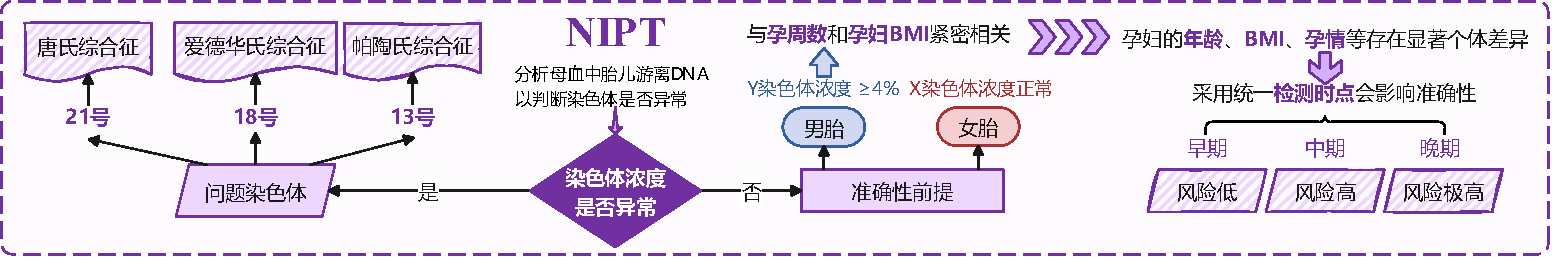
\includegraphics[width=\textwidth]{figs/1前置/问题背景.pdf}
	\caption{问题背景示意图}
\end{figure}

\section{问题重述}

\textbf{问题一:}分析胎儿染色体浓度与孕妇孕周数和身体质量指数等指标的相互关系,并建立相应的关系模型。

\textbf{问题二:}针对男胎孕妇,依据其身体质量指数进行分组,确定各组的最佳无创产前检测时点以使潜在风险最小,并分析检测误差造成的影响。

\textbf{问题三:}考虑身高,体重,年龄等多重因素与检测误差,根据男胎孕妇的身体质量指数进行分组,并给出每组的最佳无创产前检测时点,以最小化孕妇潜在风险并顾及Y染色体浓度达标比例。

\textbf{问题四:}建立女胎染色体异常的判定方法,运用Z值,GC含量,读段数及身体质量指数等多种因素,以识别21号,18号和13号染色体的非整倍体异常。


\section{问题分析(需修改)}

针对问题一,该问题涉及两个层面,其一是定性关系的判断,其二是定量规律的分析与预测。表面风化与玻璃类型、纹饰、颜色均为分类变量,它们之间的关联性分析适合采用非参数的卡方检验。风化对化学成分含量的影响则需要分组进行统计比较,通过观察含量分布的变化来识别规律。由于缺乏同一文物风化前后的成对数据,直接建立回归预测模型存在困难,因此分析的重点在于依据风化机理,构建一个基于平均变化率的风化系数模型,用以反推风化前的化学成分。

针对问题二,该问题需要从监督学习与无监督学习两个角度展开。高钾与铅钡玻璃的分类规律研究是一个典型的二分类问题,可以基于探索性数据分析发现的关键化学成分,构建支持向量机等分类模型,并对模型进行解释。

针对问题三,该问题是分类模型的实际应用与可靠性验证。分析的核心在于构建一个泛化能力强且稳健的分类器。这需要比较多种模型架构,并论证选择支持向量机的合理性。为使模型性能最优化,需要采用改进遗传算法等智能优化算法进行超参数寻优。最终的鉴别结果需要通过数据扰动和模型参数敏感性分析的双重检验,以证明其结论并非偶然,而是具有高度的可靠性。

针对问题四,该问题要求探寻不同类别玻璃内部化学成分的关联结构。由于玻璃成分数据具有总和恒定的特性,直接计算相关系数会产生误导,因此必须首先采用中心化对数比变换来消除此统计约束。直接计算相关系数会产生误导,因此必须首先采用中心化对数比变换来消除此统计约束。

全文框架如\cref{fig:全文框架}所示:

\begin{figure}[H]
	\centering
	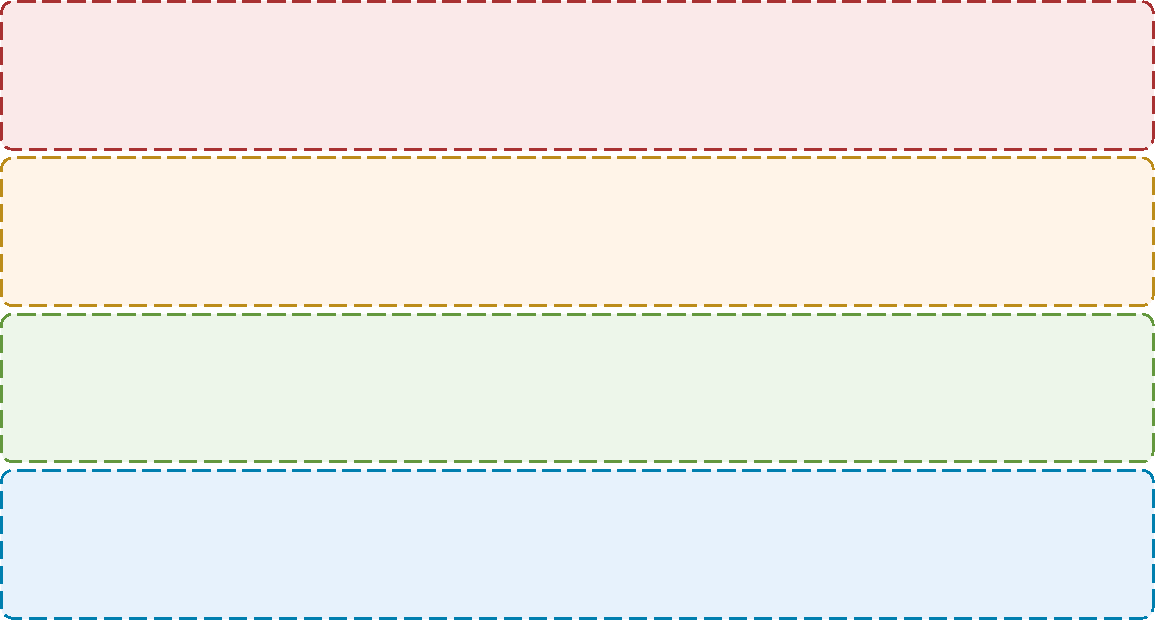
\includegraphics[width=\textwidth]{figs/1前置/全文框架.pdf}
	\caption{全文框架示意图}
	\label{fig:全文框架}
\end{figure}


\section{模型假设(需修改)}
为保证模型构建的合理性与分析过程的严谨性,我们提出以下基本假设。
\begin{enumerate}
	\item 所有用于分析的数据均为成分总和在百分之八十五至一百零五区间的有效数据。
	\item 数据中的空白项表示该化学成分未被检测到其含量可视为零。
	\item 同一类型玻璃的风化过程与化学成分变化规律具有统计上的一致性。
	\item 文物的化学成分组合能够有效地区分高钾玻璃与铅钡玻璃两大类别。
	\item 同一文物多个采样点的平均化学成分可以代表该文物的整体特征用于亚类划分。
	\item 化学成分间的偏相关关系能够反映其在玻璃配方或制作工艺中的直接关联。
	\item 化学成分间的偏相关关系能够反映其在玻璃配方或制作工艺中的直接关联。
\end{enumerate}

\section{符号说明(需修改)}
本文后续章节中所使用的主要数学符号及其说明如表所示。

\begin{table}[H]
	\centering
	\caption{符号说明表}
	\begin{tabular}{ll}
		\toprule
		\textbf{符号}                        & \textbf{说明}                     \\
		\midrule
		$k_{t,j}$                          & $t$类玻璃中$j$成分的风化系数               \\
		$\bar{C}_{t,j,\text{weathered}}$   & $t$类玻璃风化样本中$j$成分的平均含量           \\
		$\bar{C}_{t,j,\text{unweathered}}$ & $t$类玻璃未风化样本中$j$成分的平均含量          \\
		$C'_{\text{unweathered}, j}$       & 某一样本风化前$j$成分的预测含量               \\
		$\boldsymbol{w}, b$                & 支持向量机分类超平面的法向量与位移项              \\
		$C$                                & 支持向量机的正则化系数                     \\
		$\gamma$                           & 径向基核函数的参数                       \\
		$\xi_i$                            & 支持向量机的松弛变量                      \\
		$CV$                               & 变异系数,用于衡量数据的相对离散程度              \\
		$\text{clr}(\boldsymbol{x})$       & 对样本向量$\boldsymbol{x}$进行中心化对数比变换 \\
		$S$                                & 样本协方差矩阵                         \\
		$\Theta$                           & 精度矩阵,即逆协方差矩阵                    \\
		$\lambda$                          & 图套索算法的正则化参数                     \\
		$\rho_{ij \cdot \text{rest}}$      & 变量$i$和$j$之间的偏相关系数               \\
		$S$                                & 样本协方差矩阵                         \\
		$\Theta$                           & 精度矩阵,即逆协方差矩阵                    \\
		$\lambda$                          & 图套索算法的正则化参数                     \\
		$\rho_{ij \cdot \text{rest}}$      & 变量$i$和$j$之间的偏相关系数               \\
		\bottomrule
	\end{tabular}
\end{table}